\documentclass{article}
\usepackage[margin=2.5cm, includefoot, footskip=30pt]{geometry}

\setlength{\parindent}{0em}
\setlength{\parskip}{1em}
\renewcommand{\baselinestretch}{1}

%%%%Packages%%%%
\usepackage{amsmath}
\usepackage{booktabs}
\usepackage{graphics}
\usepackage{multicol}
\usepackage[ruled,vlined]{algorithm2e}
\usepackage{setspace}
\usepackage{graphicx}
\usepackage{subcaption}
\usepackage{hyperref}
\usepackage{color,colortbl}
\usepackage{array}
\usepackage{booktabs}
\usepackage{tabularx}
\usepackage{wrapfig, blindtext}
%%%%%%%%%%%%%%%%%

\definecolor{Gray}{gray}{0.92}
\usepackage[first=0,last=9]{lcg}
\newcommand{\ra}{\rand0.\arabic{rand}}

\setlength{\tabcolsep}{3pt}

\title{A meta analysis of tournaments and an evaluation of performance in the
Iterated Prisoner's Dilemma.}
\author{Nikoleta E. Glynatsi, Dr Vincent A. Knight}
\date{}

\begin{document}

\maketitle

\begin{abstract}

The Iterated Prisoner's Dilemma has been used for decades as a powerful model of
behavioural interactions. From the celebrated performance of Tit for Tat, to the
introduction of the zero-determinant strategies, to the use of sophisticated
structures such as neural networks, the literature has been exploring the
performance of strategies in the game for years. Most of these strategies are
now accessible due to an open source package; Axelrod-Python. This manuscript
make use of Axelrod-Python to conduct a meta analysis of 40000 Iterated
Prisoner's Dilemma tournaments. The aim is to evaluate the performance of
numerous strategies and finally answer the explore the factors of success in the
game.
\end{abstract}

\section{Background}

The Iterated Prisoner's Dilemma (IPD) is a repeated two player game that models
situations in which self-interest clashes with collective interest. At each turn,
the players simultaneously and independently make a choice between cooperation (C) and
defection (D) whilst having memory of the prior interactions.
The payoffs at each given turn are defined by the matrix,

\[\begin{pmatrix}
R & S \\
T & P
\end{pmatrix}\]

where \(T > R > P > S\) and \(2R > T + S\). The most common values used in
the literature~\cite{Axelrod1981}, and in this paper, are $R=3, P=1, T=5, S=0$.

Since the computer tournaments of R. Axelrod in 1980s several academic papers
are published in the field regarding the performance of strategies in the IPD.
In the 80's following the strong performance of Tit For Tat in both Axelrod's
computer tournaments~\cite{Axelrod1980a, Axelrod1980b}, and moreover in a series
of evolutionary experiments~\cite{Axelrod1981}, the strategy was thought as the
most robust basic strategy in the IPD. However, the strategy was shown to
perform poorly in environments with noise~\cite{Bendor1991, Donninger1986,
Molander1985, Hammerstein1984}. More robust strategy in such setting were
introduced and were the new protagonists, such as, Nice and
Forgiving~\cite{Bendor1991}, Pavlov~\cite{Nowak1993} and Generous Tit For
Tat~\cite{Nowak1992}.

The $20^{\text{th}}$ Anniversary Iterated Prisoner Dilemma Tournament took place
in 2004 with 233 entries. The winning strategies were based on a mechanism of
teams. A team from Southampton University took advantage of the fact that a
participant was allowed to submit multiple strategies. They submitted a total of
60 of strategies that could recognised each other and colluded to increase one
members score~\cite{J.P.Delahaye1993Lp, J.P.Delahaye1995LIeP, A.Rogers2007Ctpw}.
Yet again, in 2012 another set of strategies was introduced as the dominant set
of strategies~\cite{Press2012}. These were called zero-determinant strategies,
and by forcing a linear relationship between the payoffs they can ensure that
they will never receive less than their opponents. However, in~\cite{Harper2017}
a tournament containing over 200 strategies, zero-determinant, was performed and
none of the zero-determinant strategies ranked in top spots. Instead, the top
ranked strategies were a set of evolved strategies based lookup
tables~\cite{Axelrod1987}, hidden markov models~\cite{Harper2017} and finite
state automata~\cite{Miller1996}.
%TODO reference the archetypes of the archetypes used the IPD? Did IPD for now.

Thus, the following question is raised here: which are the true dominant
strategies in the iterated prisoner's dilemma?
This manuscript uses the open source package
Axelrod-Python~\cite{axelrodproject} to simulate a large number of computer
tournaments using as many strategies as possible from the literature. The aim is
to evaluate the performance of these strategies in a tournament and futhermore,
explore the factors of their success. This is done not for standard round robin
tournaments, but also for noisy, probabilistic ending and noisy probabilistic
ending tournaments.

The different tournaments and the data generating process are covered in
Section~\ref{section:data_collection}. Section~\ref{section:top_performances},
covers the best performed strategies for each type of tournament and overall.
Section~\ref{section:evaluation_of_performance}, explores the traits which
contribute to good performance and finally in Section~\ref{section:discussion}
the results are discussed and concluded in Section~\ref{section:conclusion}.

\section{Data generating process}\label{section:data_collection}

For the purposes of this manuscript a data set containing results on IPD tournaments
has been generated and is available at. This
was done using the open source package Axelrod-Python~\cite{axelrodproject},
more specifically, version 3.0.0. Axelrod-Python allows for different types of
IPD computer tournaments to be simulated whilst
containing a list of over 180 strategies. Most of these are strategies described
in the literature with a few exceptions being strategies that have been
contributed specifically to the package. Though Axelrod-Python features several
tournament types, this work considers only standard, noisy, probabilistic ending
and noisy probabilistic ending tournaments.

\textbf{Standard tournaments}, are tournaments similar to that of Axelrod's
in~\cite{Axelrod1980a}. There are \(N\) strategies which all play an iterated
game of \(n\) number of turns against each other. Note that self interactions
and a match against a random strategy are not included. Similarly, \textbf{noisy
tournaments} have \(N\) strategies and \(n\) number of turns but at each turn
there is a probability \(p\) that a player's action will be flipped.
\textbf{Probabilistic ending tournaments}, are of size \(N\) and after each turn
a match between strategies ends with a given probability \(e\). Finally,
\textbf{noisy probabilistic ending} tournaments have both a noise probability
\(p\) and an ending probability \(e\). For smoothing the simulated results a
tournament is repeated for \(k\) number of times. The winner of each tournament
is based on the average score a strategy achieved and not by number of wins.

%  A summary of
% each tournaments' parameters is given in Table~\ref{table:tournaments_parameters}.

% \begin{table}[!htbp]
%     \begin{center}
%         \resizebox{.85\textwidth}{!}{
%         \begin{tabular}{lcccccc}
%     \toprule
%     tournament type & number of strategies & repetitions & turns & noise probability & probability of match ending \\
%     \midrule
%     standard & $N$ & k & $n$ & - & - \\
%     noisy & $N$  & k & $n$ & $p$ & - \\
%     probabilistic ending & $N$ & k & - & - & $e$ \\
%     noisy probabilistic ending & $N$ & k & - & $p$ & $e$ \\
%     \bottomrule
%         \end{tabular}}
%     \end{center}
%     \caption{Tournament types' parameters.}
%     \label{table:tournaments_parameters}
% \end{table}

The process of generating data implemented in this manuscript is given by
Algorithm~\ref{algorithm:data_generation}. For each trial a random
size \(N\) is selected, and from the list of 186 strategies
in~\cite{axelrodproject}, a random list of \(N\) strategies is chosen. The 186
strategies used here are given in the Appendix~\ref{app:list_of_players}. For the
given list of strategies a standard, a noisy, a probabilistic ending and a noisy
probabilistic ending tournament are performed and repeated \(k\) times.
The parameters for the tournaments as well as the number of repetitions are
selected once for each trial. The parameters and their respective minimum and
maximum values are given by Table~\ref{table:parameters_values}.

\begin{table}[!htbp]
    \begin{center}
        \resizebox{.6\textwidth}{!}{
        \begin{tabular}{lcccc}
    \toprule
    parameter & parameter explanation &   min value & max value \\
    \midrule
    $N$ & number of strategies  & 3 & 195 \\
    $k$ & number of repetitions  & 10 & 100 \\
    $n$ & number of turns      & 1 & 200 \\
    $p$ & probability of flipping action at each turn  & 0 & 1   \\
    $e$ & probability of match ending in the next turn & 0 & 1   \\
    \bottomrule
        \end{tabular}}
    \end{center}
    \caption{Data generation parameters' values}
    \label{table:parameters_values}
\end{table}

The source code for the data generating process as well as the source code for
the analysis which will be discussed in the following sections have been written
following best practices~\cite{Aberdour2007, Benureau2018}. It has been packaged
and is available here.

\begin{algorithm}[!htbp]
    \setstretch{1.35}
    \ForEach{\text{seed} $\in [0, 12285]$}{
        $N \gets \text{randomly select integer}\in [N_{min}, N_{max}]$\;
        $\text{players} \gets  \text{randomly select $N$ players}$\;
        $k \gets  \text{randomly select integer}\in [k_{min}, k_{max}]$\;
        $n \gets  \text{randomly select integer}\in [n_{min}, n_{max}]$\;
        $p \gets  \text{randomly select float}\in [p_{min}, p_{max}]$\;
        $e \gets   \text{randomly select float}\in [e_{min}, e_{max}]$\;
        \vspace{0.4cm}
        $\text{result standard}$ $\gets$ Axelrod.tournament$(\text{players}, n, k)$\;
        $\text{result noisy}$ $\gets$ Axelrod.tournament$(\text{players}, n, p, k)$\;
        $\text{result probabilistic ending}$ $\gets$ Axelrod.tournament$(\text{players}, e, k)$\;
        $\text{result noisy probabilistic ending}$ $\gets$ Axelrod.tournament$(\text{players}, p, e, k)$\;

    }
    \KwRet{result standard, result noisy, result probabilistic ending,
    result noisy probabilistic ending}\;
    \caption{Data generating Algorithm}
    \label{algorithm:data_generation}
\end{algorithm}

A total of 12,285 trials of Algorithm~\ref{algorithm:data_generation} have been
performed. For each trial the results for 4 different tournaments were collected,
thus a total of 49,140 $(12,285 \times 4)$ tournament results have been
retrieved. Each tournament outputs a result summary in the form of
Table~\ref{table:output_result}.

The result summary has a length \(N\) because each row contains information for
each strategy that participated in the tournament. The information include the
strategy's rank, median score, the rate with which the strategy cooperated
$(C_r)$, it's wins and the probability that the strategy cooperated in the
opening move. Moreover, the rates of a strategy being in any of the four states
($CC, CD, DC, DD$), and the rate of which the strategy cooperated after each
state.

\newcolumntype{g}{>{\columncolor{Gray}}c}
\begin{table}[!htbp]
    \begin{center}
    \resizebox{\textwidth}{!}{
    \begin{tabular}{ccccccgcgcgcgcg}
    \toprule 
    & & & & & &   \multicolumn{8}{g}{Rates}  \\
    Rank & Name & Median score & Cooperation rating $(C_r)$ & Win & Initial C &
    CC & CD & DC & DD & CC to C & CD to C & DC to C & DD to C \\
    0 &  EvolvedLookerUp2 2 2 & 2.97 & 0.705 & 28.0 & 1.0 & 0.639 & 0.066 & 0.189 &
    0.106 & 0.836 & 0.481 & 0.568 & 0.8 \\
    1 &  Evolved FSM 16 Noise 05 & 2.875 & 0.697 & 21.0 & 1.0 & 0.676 & 
    0.020 & 0.135 & 0.168 & 0.985 & 0.571 & 0.392 & 0.07 \\
    2 & PSO Gambler 1 1 1 & 2.874 & 0.684 &  23.0 &     1.0 &    0.651 &    0.034 &    0.152 &    0.164
    & 1.000 & 0.283 & 0.000 & 0.136 \\
    3 &  PSO Gambler Mem1 &  2.861 &        0.706 &  23.0 &      1.0 &    0.663
    &    0.042 &    0.145 &    0.150 &  1.000 &  0.510 &  0.000 &  0.122 \\
    4 &          Winner12 &  2.835 &        0.682 &  20.0 &      1.0 &
    0.651 &    0.031 &    0.141 &    0.177 &  1.000 &  0.441 &  0.000 &  0.462 \\
    $\dots$ & $\dots$ & $\dots$ & $\dots$ & $\dots$ & $\dots$ & $\dots$ & $\dots$ &
    $\dots$ & $\dots$ & $\dots$ & $\dots$ & $\dots$ & $\dots$ \\
    \bottomrule
    \end{tabular}}
\end{center}
\caption{Output result.}\label{table:output_result}
\end{table}

The \textbf{normalised rank} is a measure which was manually included. The normalised
rank, denoted as $r$, is calculated as a strategy's rank divided by the
tournament's size ($N$). The normalised rank will be used in the next section to
evaluate the performance of strategies.

\section{Top ranked strategies}\label{section:top_performances}

This section evaluates the performance of 186 strategies. The performance of
each strategy will be evaluated for each type of tournament independently,
followed by an evaluation of their performance over all the simulated
tournaments of this work. Each strategy could have participated in multiple
tournaments of the same type (on average each participated in 5690 different
tournaments). For example Tit For Tat has participated in a total of 5569
tournaments of each type. The strategy's normalised rank distribution in these
is given in Figure~\ref{fig:tit_for_tat_r_distribution}. As a result, of the
multiple entries of strategies their performance is evaluated based on the
\textbf{median normalised rank} denoted as \(\bar{r}\). A value of \(\bar{r} =
0\) corresponds to a strategy winning the tournament where a a value of
\(\bar{r} = 1\) corresponds to the strategy coming last.

\begin{figure}[!htbp]
    \centering
    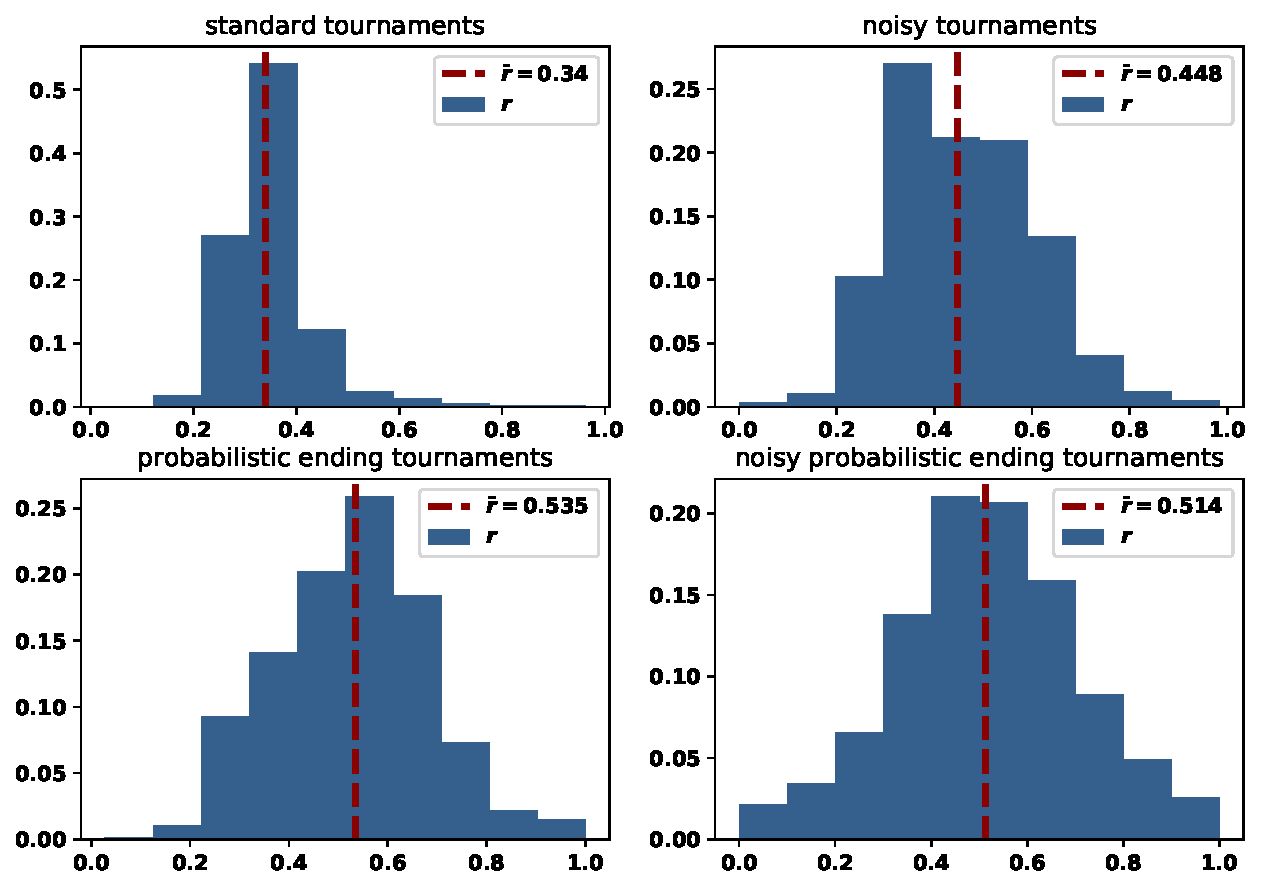
\includegraphics[width=.8\textwidth]{../images/tit_for_tat_r_distributions.pdf}
    \caption{Tit For Tat's $r$ distribution in tournaments. The best performance
    of the strategy has been in standard tournaments where it achieved a normalised
    rank of 0.339.}
    \label{fig:tit_for_tat_r_distribution}
\end{figure}

The result of each tournament type are based on $12,285$ trials. The strategies
are ranked based on the median normalised rank they achieved and the top 15
strategies of each tournament are given in Table~\ref{table:top_performances}.


\newcolumntype{g}{>{\columncolor{Gray}}l}
\begin{table}[!htbp]
    \begin{center}
    \resizebox{.9\textwidth}{!}{
        \begin{tabular}{lggllggllr}
\toprule
& \multicolumn{2}{g}{Standard} & \multicolumn{2}{c}{Noisy} & \multicolumn{2}{g}{Probabilistic ending} &  \multicolumn{2}{c}{Noisy probabilistic ending} \\
\midrule
& Name & $\bar{r}$ &                 Name & $\bar{r}$ &               Name & $\bar{r}$ &                 Name & $\bar{r}$ \\
\midrule
1 &           Evolved HMM 5 &   0.00667 &               Grumpy &    0.1402 &          Fortress4 &   0.01266 &           Alternator &    0.3037 \\
2 &          Evolved FSM 16 &   0.00995 &                  $e$ &   0.19388 &           Defector &   0.01429 &               $\phi$ &   0.30978 \\
3 &    EvolvedLookerUp2 2 2 &   0.01064 &       Tit For 2 Tats &    0.2069 &  Better and Better &   0.01587 &                  $e$ &    0.3125 \\
4 & Evolved FSM 16 Noise 05 &   0.01667 &         Cycle Hunter &   0.21538 &    Tricky Defector &   0.01875 &                $\pi$ &   0.31686 \\
5 &       PSO Gambler 2 2 2 &   0.02143 &       Risky QLearner &   0.22222 &          Fortress3 &   0.02174 &    Limited Retaliate &   0.35263 \\
6 &             Evolved ANN &   0.02878 &          Retaliate 3 &   0.22887 &     Gradual Killer &   0.02532 &     Anti Tit For Tat &   0.35431 \\
7 &           Evolved ANN 5 &    0.0339 &        Cycler CCCCCD &   0.23507 &         Aggravater &   0.02778 &          Retaliate 3 &   0.35563 \\
8 &       PSO Gambler 1 1 1 &   0.03704 &          Retaliate 2 &   0.23913 &             Raider &   0.03077 &  Limited Retaliate 3 &   0.35563 \\
9 &           Evolved FSM 4 &   0.04891 &      Defector Hunter &   0.24038 &         Cycler DDC &   0.04545 &            Retaliate &   0.35714 \\
10 &        PSO Gambler Mem1 &   0.05036 &            Retaliate &   0.24177 &        Hard Prober &   0.05128 &          Retaliate 2 &   0.35767 \\
11 &                Winner12 &   0.06011 &  Hard Tit For 2 Tats &      0.25 &         SolutionB1 &   0.06024 &  Limited Retaliate 2 &   0.36134 \\
12 &            Fool Me Once &    0.0614 &             ShortMem &   0.25286 &      Meta Minority &   0.06077 &             Hopeless &   0.36842 \\
13 &                     DBS &   0.07143 &  Limited Retaliate 3 &   0.25316 &              Bully &   0.06081 &    Arrogant QLearner &   0.40651 \\
14 &           DoubleCrosser &     0.072 &    Limited Retaliate &   0.25706 &    Fool Me Forever &    0.0708 &    Cautious QLearner &   0.40909 \\
15 &             BackStabber &   0.07519 &                $\pi$ &   0.25801 &             EasyGo &   0.07101 &      Fool Me Forever &   0.41764 \\
\bottomrule
    \end{tabular}
    
    }
\end{center}
\caption{Top performances for each tournament type based on $\bar{r}$.}
\label{table:top_performances}
\end{table}

In standard tournaments 10 of the 15 top strategies are strategies introduced
in~\cite{Harper2017}. These have been trained using reinforcement learning
algorithms and are based on finite state automata (FSM), hidden markov models
(HMM), artificial neural networks (ANN), lookup tables (LookerUp) and stochastic
lookup tables (Gambler). Specifically, the have been trained against the
strategy list of~\cite{axelrodproject} in standard tournaments. Thus their
performance is to be expected. DoubleCrosser, and Fool Me Once, are not from the
literature but from~\cite{axelrodproject}. DoubleCrosser is a strategy that
makes use of the length of the match because is set to defect on the last two
rounds. The strategy is expected to not perform as well in probabilistic ending
tournaments. Finally, Winner 12~\cite{mathieu2017} and DBS are both from the the
literature. DBS~\cite{Au2006} is strategy specifically designed for noisy
environments, however, it ranks highly only in standard ones.

Figure~\ref{fig:std_results} gives the distributions of $\bar{r}$ for the top
ranked strategies. The distributions are skewed towards zero and the highest
median is at 0.075. This indicates that the top ranked strategies are dominating
strategies in standard tournaments. They are very likely to perform well in
standard tournament despite the number of opponents, the opponents, the turns
etc. This does not hold for all the tournament types as it will be discussed
in the later parts.

\begin{figure}[!htbp]
    \centering
    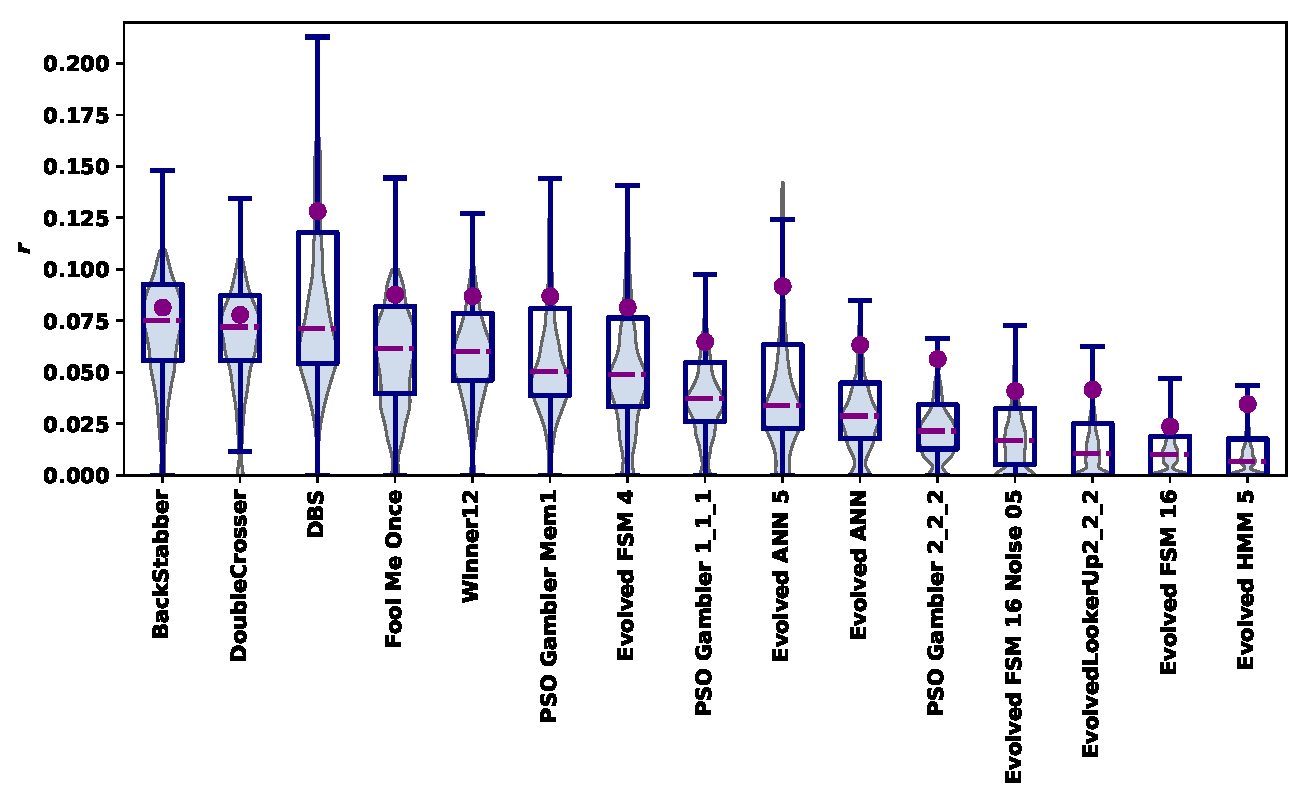
\includegraphics[width=.7\textwidth]{../images/performance_standard.pdf}
    \caption{$\bar{r}$ distributions of top 15 strategies in standard tournaments.}\label{fig:std_results}
\end{figure}

The top strategies in noisy tournaments include the two strategies, Tit For 2
Tats~\cite{Axelrod1980b} and Hard Tit For 2 Tats~\cite{Stewart2012}, which are
strategies that will defect only after the have received two defections from the
opponent. The Retaliate strategies are set of strategies
from~\cite{axelrodproject} that start by cooperating but will retaliate once the
opponent's wins and defections surpass a curtain threshold.
ShortMem~\cite{Carvalho2013}, Grumpy, $e$ and $\phi$ are strategies that make
decisions based on the cooperations to defections ratio. In $5^{\text{th}}$ and
$6^{\text{th}}$ place are the strategies Cycler Hunter and  Risky QLearn. Cycler
Hunter tries to extort strategies that play cyclically and Risky QLearn uses a Q
learning algorithm. Notably, a deterministic and one of the most simple
strategies in game is ranked $3^{\text{rd}}$. That is Cooperator, a strategy
that just cooperates.

From Figure~\ref{fig:std_results} it is evident that the normalised rank distributions
in noisy environments are more variant and have higher median values compared
to standard tournaments. The distributions are skewed both towards
0 and 1 which indicates that though the top ranked strategies mainly
performed well (medians $< 0.3$) there are several tournaments that they performed
worse than the 60\% of the participants.

\begin{figure}[!htbp]
    \centering
    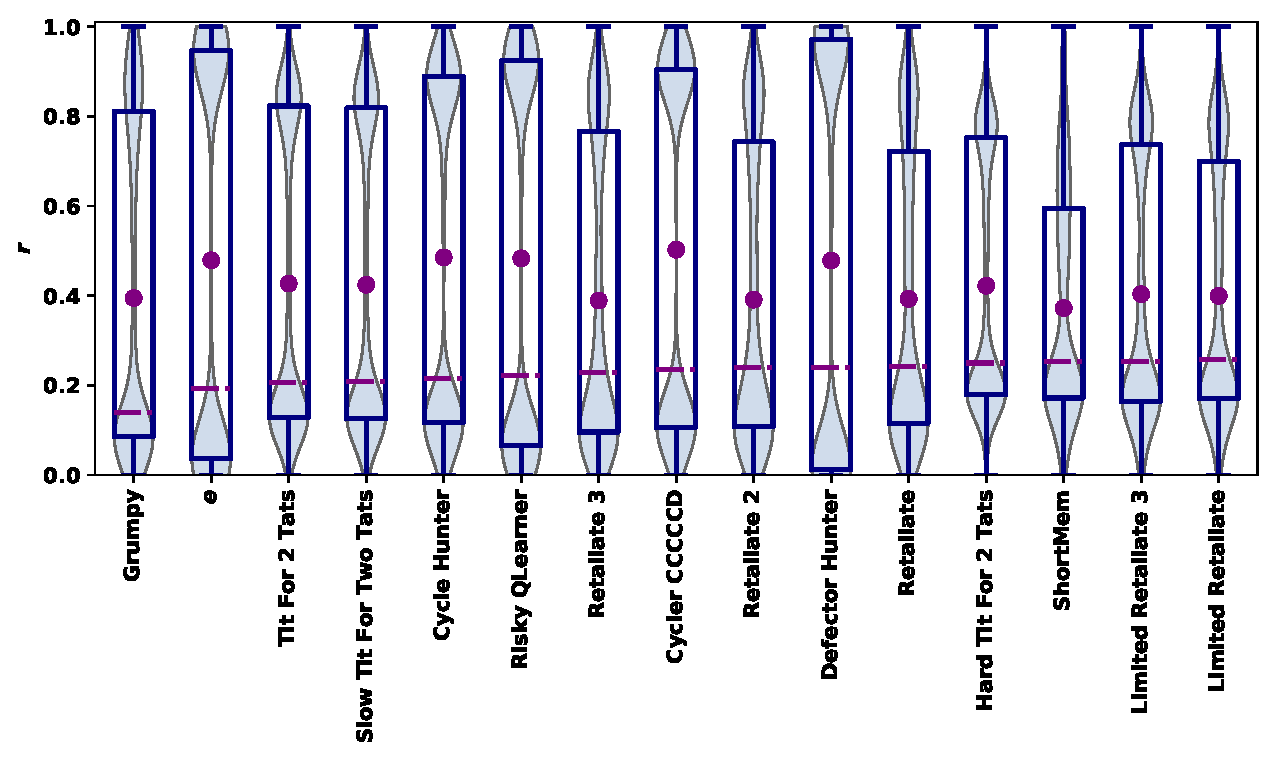
\includegraphics[width=.7\textwidth]{../images/performance_noise.pdf}
    \caption{\(\bar{r}\) distributions for best performed strategies in noisy tournaments.}
    \label{fig:noisy_results}
\end{figure}

The 15 top ranked strategies in probabilistic ending tournaments include
Fortress 3, Fortress 4 (both introduced in~\cite{Ashlock2006}),
Raider~\cite{Ashlock2014} and Solution B1~\cite{Ashlock2014} which are strategies
based on finite state automata introduced by Daniel and Wendy Ashlock. These
strategies have been evolved using reinformed learning, however, there were
trained to maximise their payoffs in tournaments with fixed turns (150
specifically) and not in probabilistic ending ones.
In probabilistic ending tournaments it appears that the top ranks are mostly
occupied by defecting strategies which include Better and Better, Gradual
Killer, Hard Prober (all from ~\cite{prison}), Bully (Reverse Tit For
Tat)~\cite{Nachbar1992} and Defector. Thus, it's surprisingly that EasyGo and
Fool Me Forever are ranked $14^{\text{th}}$ and $15^{\text{th}}$. These
strategies are actually the same; they will defect until their opponent defect,
then they will cooperate until the end. Both strategies have repeatedly ranked highly
as shown in Figure~\ref{fig:probend_results} and there are cases for which they
were the winners of the tournament.

The distributions of the normalised rank in probabilistic ending tournaments are
less variant than those of noisy tournaments. The medians are lower than 0.1 and the
distributions are skewed towards 0. Though the large difference between the means
and the medians indicates some outliers, the strategies have overall performed
well in the tournaments that they participated.

\begin{figure}[h!]
    \centering
    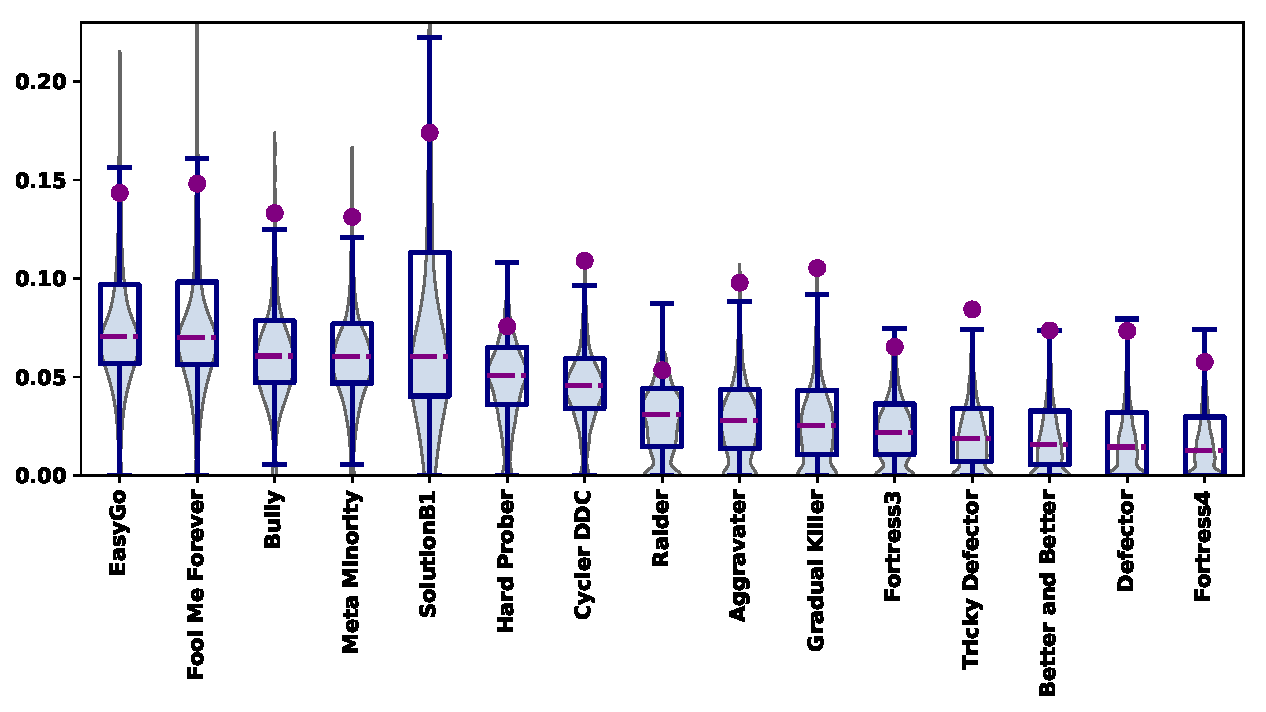
\includegraphics[width=.7\textwidth]{../images/performance_probend.pdf}
    \caption{\(\bar{r}\) distributions for best performed strategies in probabilistic ending tournaments.}
    \label{fig:probend_results}
\end{figure}

In tournaments that have both noise and an unspecified number of turns several
of the top ranked strategies are strategies that were highly ranked in
noisy tournaments as well. However, strategies from the top ranks of
probabilistic ending tournaments did not rank highly here. The Retaliate set,
$\phi, e$ and Anti Tit For Tat behaviour strategies appear to perform well in
noisy environments. So these strategies performed well in this setting as well
even though now the turns are not specified.
The top ranked strategy is Alternator a strategy that alternate between
cooperation and defection. Hopeless~\cite{Van2015} is a strategy that will only
defect if and only if a mutual cooperation and the last three places are
occupied by strategies based on a Q learning algorithm. The three Q learning
strategies are the only ones that have bimodal distributions of normalised
ranks. In comparison, the rest of the distributions are skewed towards
0.4, Figure~\ref{fig:noisy_probend_results}.

\begin{figure}[!htbp]
    \centering
    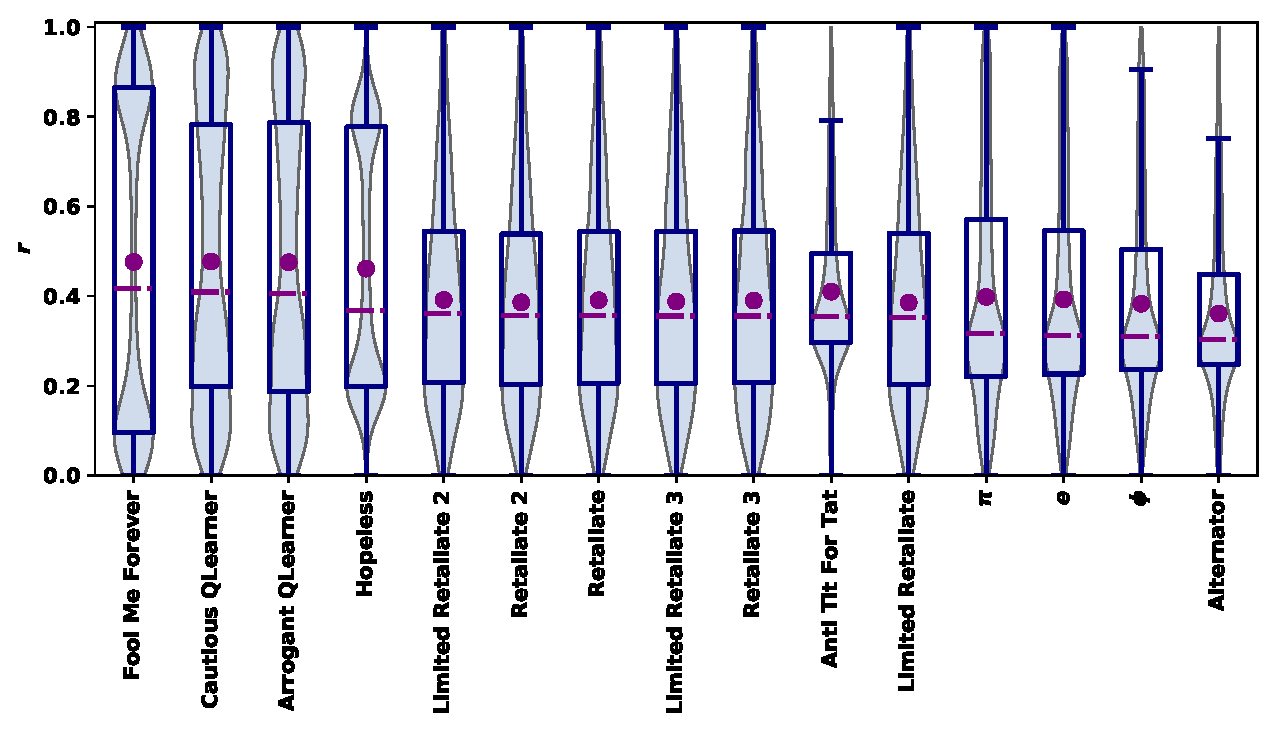
\includegraphics[width=.7\textwidth]{../images/performance_probend_noise.pdf}
    \caption{\(\bar{r}\) distributions for best performed strategies in noisy
    probabilistic ending tournaments.}
    \label{fig:noisy_probend_results}
\end{figure}

\begin{table}[!htbp]
    \centering
    \resizebox{.35\textwidth}{!}{
    \begin{tabular}{lr}
\toprule
{} &  Normalized\_Rank \\
Name                    &                  \\
\midrule
Evolved FSM 16          &            0.018 \\
Evolved HMM 5           &            0.019 \\
Evolved FSM 16 Noise 05 &            0.025 \\
EvolvedLookerUp2\_2\_2    &            0.028 \\
Evolved ANN             &            0.037 \\
PSO Gambler 2\_2\_2       &            0.040 \\
Evolved ANN 5           &            0.046 \\
PSO Gambler 1\_1\_1       &            0.061 \\
Fool Me Once            &            0.067 \\
Evolved FSM 4           &            0.075 \\
DoubleCrosser           &            0.079 \\
Winner12                &            0.081 \\
BackStabber             &            0.082 \\
DBS                     &            0.086 \\
PSO Gambler Mem1        &            0.089 \\
\bottomrule
\end{tabular}
}
    \caption{Top performances in data set}\label{table:overall_results}
\end{table}

So far the performances have been evaluated separately for each tournament
type. The merged data set, which was described in Section~\ref{section:data_collection},
contains a total of 49,140 result summaries. The 15 top ranked strategies
overall are given in Table~\ref{table:overall_results}. The top ranks
include strategies that have been mentioned before due to their performance
in specific tournaments. The top ranks are overtaken by the set of Retaliate
strategies followed by BackStabber and DoubleCrosser. DoubleCrosser performed
well in standard tournaments and the strategy is just an extension of BackStabber.
The two strategies Nice Meta Winner and NMWE Memory One are strategies based on teams.
PSO Gambler and Evolved HMM 5 are trained strategies introduced in~\cite{Harper2017}
and Stein and Rapoport and Grudger are strategies from Axelrod's
original tournament where they came 6th and 7th respectively. Forgetful Fool Me
Once is based on the same approach as Grudger.

Figure~\ref{fig:overall_results} gives the normalised rank distributions
of these strategies. It is evident that the Retaliate strategies performances
are very similar and their distributions are different in comparison with the
rest of the top ranked strategies in the setting.

\begin{figure}[!htbp]
    \centering
    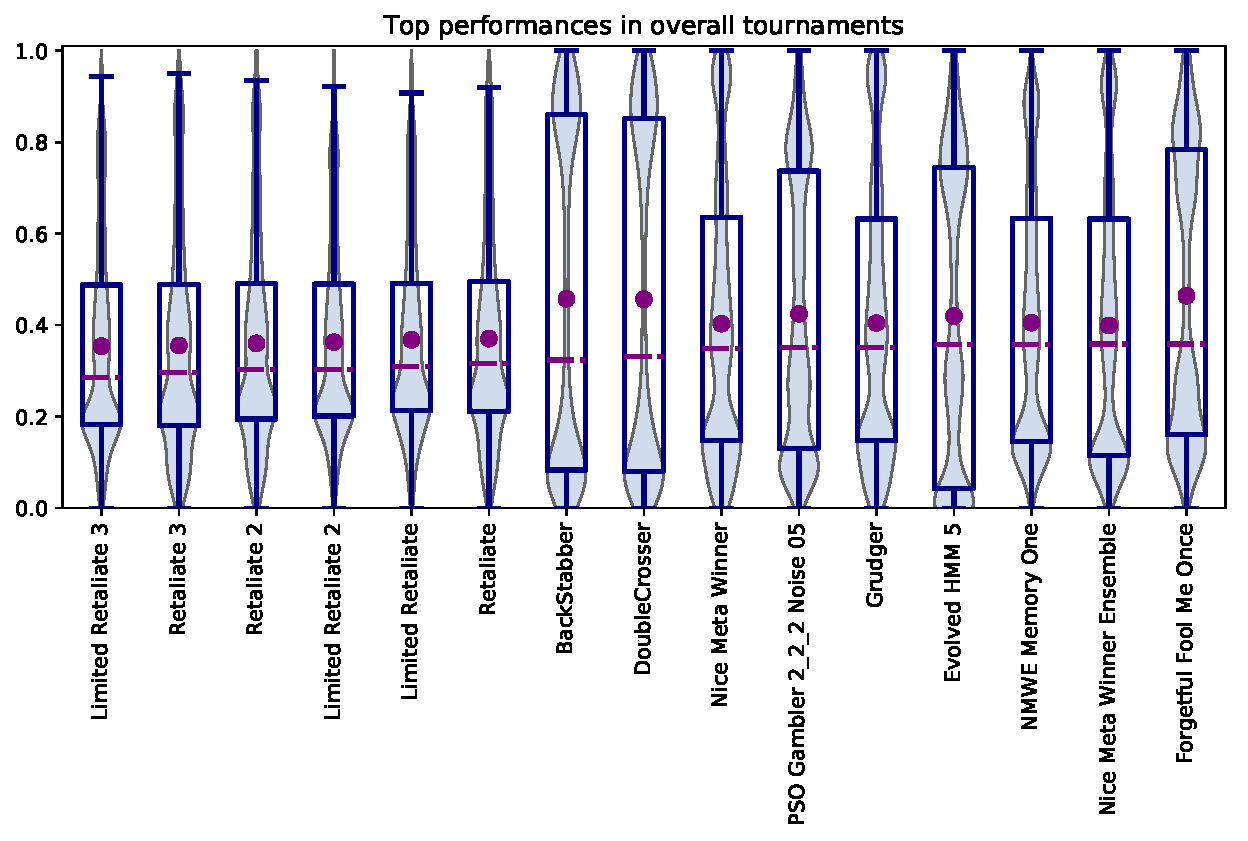
\includegraphics[width=.8\textwidth]{../images/performance_merged.pdf}
    \caption{\(\bar{r}\) distributions for best performed strategies in data set.}
    \label{fig:overall_results}
\end{figure}

This section presented the top ranked performances.

\begin{itemize}
    \item In standard tournaments the top ranked spots were dominated by complex
    strategies that have been trained using reinforcement learning techniques.
    These strategies dominated most the tournaments that have been involved in.
    \item In noisy tournaments the top ranked strategies were all different to those of standard
    tournaments. Most of the top ranked strategies were basing their decisions
    on the he defection to cooperation ratio. These
    strategies had won most the tournaments in which they participated, however,
    they also ranked last in several tournaments.
    \item Once again in probabilistic ending tournaments the top ranked
    strategies were different to those before. More defecting strategies
    occupied the top ranks in this setting, as well as finite state automata
    that have been introduced all by the same authors.
    \item Moreover, in noisy probabilistic ending tournaments it was the only
    set of tournaments were the highly ranked strategies have been covered
    before, more specifically, in noisy tournaments. In these tournaments the
    means and medians of the distributions were close to 0.4. Indicating that on
    average these strategies managed to consistently perform on the top 40\% of
    the strategies.
    \item Finally, using all the tournaments results, despite their type, the top
    ranked strategies were a mixture of behaviours that do well in standard
    tournaments and tournaments with noise. The top ranks also included two
    strategies that are based on teams.
\end{itemize}

In this section the winning strategies in a series of IPD tournaments of
different settings were presented. Though there have been instances of
strategies that do well in more than one setting, most of the top ranks were
occupied by different strategies each time. The top ranks have been occupied
by strategies with small memory size, with infinite memory size, sophisticated
and deterministic strategies. Even two of the most basic strategic rules,
Cooperator and Defector, have been ranked in the top 15 places.

This indicates that in an IPD tournament a winning strategy exist but only for
the given environment, however, there is no dominant strategy in the IPD that
can do well in any tournament where the settings can vary. The aim of the next
section is to understand which are the factors that made these strategies
successful. In each setting separately but also overall.

\section{Evaluation of performance}\label{section:evaluation_of_performance}

The aim of this section is to explore the factors that contribute to a
strategy's successful performance. The factors explored are measures regarding a
strategy's behaviour but also measures regarding the tournaments the strategies
competed in. More specifically the factors that are included in the analysis are
given by Table~\ref{table:manual_measures} and
Table~\ref{table:parameters_values}.

Axelrod-Python makes use of classifiers to classify strategies according to
various dimensions. The classifiers considered in this work are the stochastic
classifier, the make use of game and length classifiers. These determine whether
a strategy is stochastic or deterministic, whether it makes use of the number of
turns or the game's payoffs. The SSE is a measure extortionate
behaviour introduced in~\cite{Knight2019}. A value of 1 indicates no
extortionate behaviour at all whereas a value of 0 indicates that a strategy is
always trying to extortion the opponent. The rest of the factors considered
are the $CC$ to $C$, $CD$ to $C$, $DC$ to $C$, and $DD$ to $C$ rates as well as
cooperating ratio of a strategy. The minimum, maximum, medium and median
cooperating ratios of each tournament are also included, and finally the number of
turns, the size and the probabilities of noise or the game ending.

\newcolumntype{g}{>{\columncolor{Gray}}c}
\begin{table}[h]
    \begin{center}
    \resizebox{\textwidth}{!}{
    \begin{tabular}{gcgcgc}
    \toprule
    measure & measure explanation &  source & value type & min value & max value \\
    \midrule
stochastic  &  If a strategy is stochastic & strategy classifier from~\cite{axelrodproject} & boolean  & False &  True \\
makes use of game &  If a strategy makes used of the game information & strategy classifier from~\cite{axelrodproject} & boolean  & False &  True \\
makes use of length &  If a strategy makes used of the number of turns & strategy classifier from~\cite{axelrodproject} & boolean  & False &  True \\
SSE & A measure of how far a strategy is from extortionate behaviour & method described in~\cite{Knight2019} & float & 0 & 1 \\
max cooperating rate $(C_{\text{max}})$  & The biggest cooperating rate in the tournament & result summary & float & 0 & 1 \\
min cooperating rate $(C_{\text{min}})$ & The smallest cooperating rate in the tournament & result summary & float & 0 & 1 \\
median cooperating rate $(C_{\text{median}})$ & The median cooperating rate in the tournament & result summary & float & 0 & 1 \\
mean cooperating rate $(C_{\text{mean}})$ & The mean cooperating rate in the tournament & result summary & float & 0 & 1 \\
$C_r$ / $C_{\text{max}}$ & A strategy's cooperating rate divided by the maximum & manually & float & 0 & 1 \\
$C_r$ / $C_{\text{min}}$ & A strategy's cooperating rate divided by the minimum & manually & float & 0 & 1 \\
$C_r$ / $C_{\text{median}}$ & A strategy's cooperating rate divided by the median & manually & float & 0 & 1 \\
$C_r$ / $C_{\text{mean}}$ & A strategy's cooperating rate divided by the mean & manually & float & 0 & 1 \\
$C_r$ & The cooperating ratio of a strategy & result summary & float & 0 & 1 \\
$CC$ to $C$ rate & The probability a strategy will cooperate after a mutual cooperation & result summary & float & 0 & 1 \\
$CD$ to $C$ rate & The probability a strategy will cooperate after being betrayed by the opponent & result summary & float & 0 & 1 \\
$DC$ to $C$ rate & The probability a strategy will cooperate after betraying the opponent & result summary & float & 0 & 1 \\
$DD$ to $C$ rate & The probability a strategy will cooperate after a mutual defection & result summary & float & 0 & 1 \\
    \bottomrule
        \end{tabular}}
    \end{center}
    \caption{Manually calculated/retrieved measures.}
    \label{table:manual_measures}
\end{table}

%memory depth &  Strategy's memory size & strategy classifier from~\cite{axelrodproject} & integer & 0 & $\infty$ \\

The effect of these factors on a strategy's success is evaluated based on the
correlation coefficient between the factors, the normalised rank and the median
score. The correlation coefficients are given by Table~\ref{table:correlations}.
Note that the correlation for the classifiers is not included because they are
binary variables and they will evaluated by a different method. 

% The
% correlations of each factor against each factor, the normalised rank and the
% median are also given in the Appendix.

\newcolumntype{g}{>{\columncolor{Gray}}c}
\begin{table}[!htbp]
    \begin{center}
    \resizebox{.8\textwidth}{!}{
        \begin{tabular}{lggccggccggg}
    \toprule
    &  \multicolumn{2}{g}{Standard} & \multicolumn{2}{c}{Noisy} & \multicolumn{2}{g}{Probabilistic ending} &  \multicolumn{2}{c}{Noisy probabilistic ending} &  \multicolumn{2}{g}{Overall} \\
\midrule
{} &  $r$ &  median score &  $r$ &  median score &  $r$ &  median score &  $r$ &  median score &  $r$ &  median score\\
\midrule
$CC$ to $C$ rate     & -0.501 &  0.501 &   0.414 &  -0.504 &   0.408 &  -0.323 &   0.260 &   0.022 &  -0.501 &  0.501 \\
$CD$ to $C$ rate     &  0.226 & -0.199 &   0.456 &  -0.330 &   0.320 &  -0.017 &   0.205 &  -0.220 &   0.226 & -0.199 \\
$C_r$                & -0.323 &  0.384 &   0.711 &  -0.678 &   0.714 &  -0.832 &   0.579 &  -0.135 &  -0.323 &  0.384 \\
$C_r$ / $C_{max}$    & -0.323 &  0.381 &   0.616 &  -0.551 &   0.714 &  -0.833 &   0.536 &  -0.116 &  -0.323 &  0.381 \\
$C_r$ / $C_{mean}$   & -0.331 &  0.358 &   0.731 &  -0.740 &   0.721 &  -0.861 &   0.649 &  -0.621 &  -0.331 &  0.358 \\
$C_r$ / $C_{median}$ & -0.331 &  0.353 &   0.652 &  -0.669 &   0.712 &  -0.852 &   0.330 &  -0.466 &  -0.331 &  0.353 \\
$C_r$ / $C_{min}$    &  0.109 & -0.080 &  -0.358 &   0.250 &  -0.134 &   0.150 &  -0.368 &   0.113 &   0.109 & -0.080 \\
$C_{max}$            & -0.000 &  0.049 &   0.000 &   0.023 &  -0.000 &   0.046 &   0.000 &  -0.004 &  -0.000 &  0.049 \\
$C_{mean}$           & -0.000 &  0.229 &  -0.000 &   0.271 &   0.000 &   0.200 &   0.000 &   0.690 &  -0.000 &  0.229 \\
$C_{median}$         &  0.000 &  0.209 &  -0.000 &   0.240 &  -0.000 &   0.187 &  -0.000 &   0.673 &   0.000 &  0.209 \\
$C_{min}$            &  0.000 &  0.084 &   0.000 &  -0.017 &  -0.000 &   0.007 &  -0.000 &   0.041 &   0.000 &  0.084 \\
$DC$ to $C$ rate     &  0.127 & -0.100 &   0.509 &  -0.504 &  -0.018 &   0.033 &   0.341 &  -0.016 &   0.127 & -0.100 \\
$DD$ to $C$ rate     &  0.412 & -0.396 &   0.533 &  -0.436 &  -0.103 &   0.176 &   0.378 &  -0.263 &   0.412 & -0.396 \\
$N$                  &  0.000 & -0.009 &  -0.000 &   0.002 &  -0.000 &   0.003 &  -0.000 &   0.001 &   0.000 & -0.009 \\
$k$                  &  0.000 & -0.002 &  -0.000 &   0.003 &  -0.000 &   0.001 &  -0.000 &  -0.008 &   0.000 & -0.002 \\
$n$                  &  0.000 & -0.125 &  -0.000 &  -0.024 &       - &       - &       - &       - &   0.000 & -0.125 \\
$p_e$                &      - &      - &        - &     - &    0.000 &   0.165 &   0.000 &  -0.058 &  -0.001 &  0.001 \\
$p_n$                &      - &      - &  -0.000 &   0.207 &       - &       - &  -0.000 &  -0.650 &   0.002 & -0.000 \\
Make use of game     & -0.003 & -0.022 &   0.025 &  -0.082 &  -0.053 &  -0.108 &   0.013 &  -0.016 &  -0.003 & -0.022 \\
Make use of length   & -0.158 &  0.124 &   0.005 &  -0.123 &  -0.025 &  -0.090 &   0.014 &  -0.016 &  -0.154 &  0.117 \\
SSE                  &  0.473 & -0.452 &   0.463 &  -0.337 &  -0.156 &   0.223 &   0.305 &  -0.259 &   0.473 & -0.452 \\
memory usage         & -0.082 &  0.095 &  -0.007 &  -0.017 &       - &     - &     - &           - &  -0.084 &  0.095 \\
stochastic           &  0.006 & -0.024 &   0.022 &  -0.026 &   0.002 &  -0.130 &   0.021 &  -0.013 &   0.006 & -0.024 \\
\bottomrule
\end{tabular}

    }
\end{center}
\caption{Correlations table.}\label{table:correlations}
\end{table}

In standard tournaments the measures  $CC$ to $C$, $C_r$, $C_r / C_{\text{max}}$
and the cooperating ratio compared to the median and the mean have a moderate
negative effect on the normalised rank and a moderate positive on the median
score. The SSE error and the $DD$ to $C$ have the opposite effects. Thus, in
standard tournaments behaving cooperative corresponds to a more successful
performance. However, even though being cooperative pays of that's not true
against defective strategies. Cooperating after a mutual defection lowers a
strategy's success. Figure\ref{fig:rates_of_winners_in_standard_tournaments}
confirms these. The winner of standard tournaments almost always cooperated
after a mutual cooperation but the 50\% only cooperated with a probability
of 0.2 after a mutual defection.

\begin{figure}[!htbp]
    \centering
    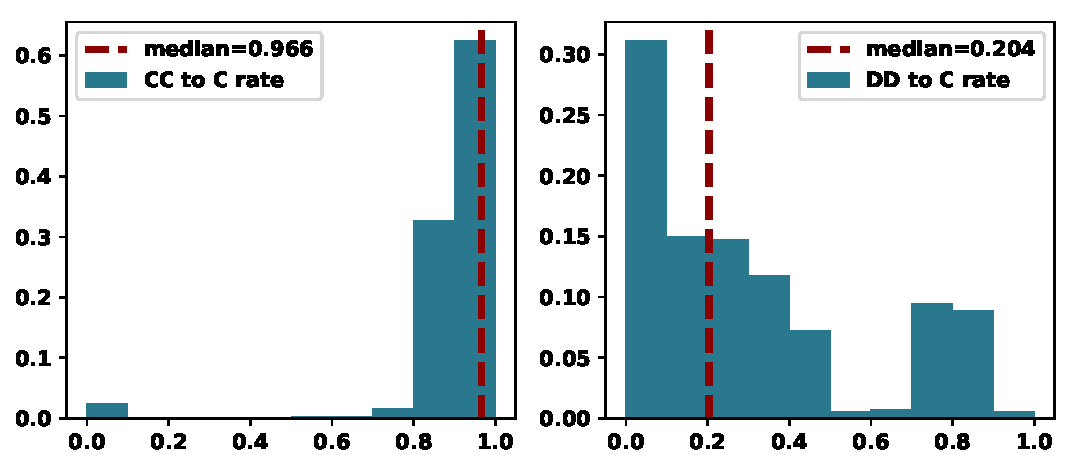
\includegraphics[width=.7\textwidth]{../images/rates_of_winners_in_standard_tournaments.pdf}
    \caption{Winners distributions
    in standard tournaments for $CC$ to $C$ and $DD$ to $C$.}\label{fig:rates_of_winners_in_standard_tournaments}
\end{figure}

Compared to standard tournaments in both noisy and in probabilistic ending
tournaments the higher the rates of cooperation the lower a strategy's success
and median score. Moreover, a strategy would want to cooperate less than both
the mean and median cooperator in such settings. In probabilistic ending
tournaments the correlations coefficients have a larger values, indicating a
stronger effect. Thus a strategy will be punished more by it's cooperative
behaviour in such environments. The distributions of the $C_r$ of the winners in
both tournaments is given by Figure~\ref{fig:c_r_distributions}. It confirms
that the winners in these two settings were more defective strategies, mainly
in probabilistic ending ones.

\begin{figure}[!htbp]
    \centering
    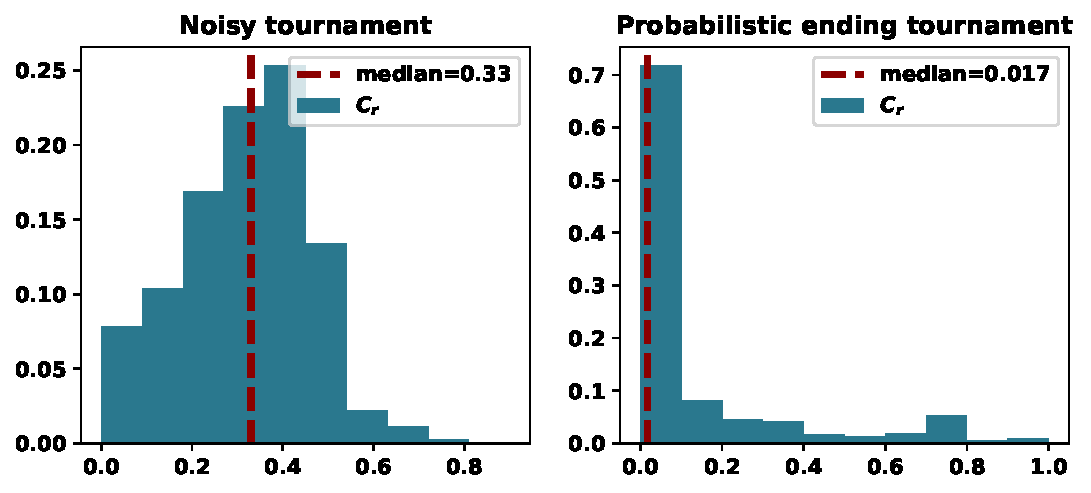
\includegraphics[width=.7\textwidth]{../images/c_r_winners_tournaments.pdf}
    \caption{$C_r$ distributions.}\label{fig:c_r_distributions}
\end{figure}

In noisy probabilistic ending tournaments and in the overall tournaments the
only factors that had a moderate affect are $C_r/C_{\text{mean}},
C_r/C_{\text{max}}$ and $C_r$. In such environments cooperative behaviour
appears to be punished by not as much as in noisy and probabilistic ending
tournaments.

To further evaluate the effect of factors on performances a random forest
classification~\cite{breiman2001} is applied. Initially, the performances are
clustered based on their normalised rank and the median score by a \(k-\)means
algorithm~\cite{Arthur2007}. The number of clusters are not deterministically
chosen but are based on the silhouette coefficients~\cite{Rousseeuw1987}.
Consider the case of standard tournaments, the chosen number of clusters is
2 and Figure~\ref{fig:standard_clusters} illustrates the trials of clustering the
performances in 2, 3 and 4 clusters respectively. The number of chosen clusters
for each type and overall are given in Table~\ref{table:number_of_clusters}.

\begin{figure}[!htbp]
\centering
\includegraphics[width=.7\textwidth]{../output/standard/clusters_plots.png}
\caption{Clustering trials for standard tournaments. A number of 2 clusters has
been chosen with a silhouette score of  0.66 against 0.511 and 0.50
respectively.}\label{fig:standard_clusters}
\end{figure}

\begin{table}[!htbp]
    \begin{center}
        \resizebox{.5\textwidth}{!}{
        \begin{tabular}{lcccc}
    \toprule
    type & number of clusters &  silhouette coefficient\\
    \midrule
    standard                   & 2 & 0.648 \\
    noisy                      & 3 & 0.493 \\
    probabilistic ending       & 2 & 0.680 \\
    noisy probabilistic ending & 4 & 0.415\\
    overall                    & 3 & 0.443\\
    \bottomrule
        \end{tabular}}
    \end{center}
    \caption{Number of clusters for each type and overall and the respective silhouette coefficients.}
    \label{table:number_of_clusters}
\end{table}

A random forest approach is applied to the data to predict the cluster to which
a strategy's performance has been assigned to. The random forest method
constructs many individual decision trees and the predictions from all trees are
pooled to make the final prediction. The random forest models are trained on a
training set of 70\% of the tournaments results. The accuracy of each model
based on $R^2$ are given by Table~\ref{table:accuracy_random_forest}. The out of
the bag error~\cite{hastie2005} has also been calculated. The models fit well and
the values of the accuracy measures on the test data and the OOB error indicate that they are not
over fitting.

\begin{table}[!htbp]
    \begin{center}
        \resizebox{.5\textwidth}{!}{
        \begin{tabular}{lcccc}
    \toprule
    type & $R^2$ training data &  $R^2$ test data  & $R^2$ OBB score\\
    \midrule
    standard                   & 0.998545  & 0.989890 & 0.982331\\
    noisy                      & 0.996677  & 0.950572 & 0.935383\\
    probabilistic ending       & 0.999592  & 0.995128 & 0.992819 \\
    noisy probabilistic ending & 0.990490  & 0.813905 & 0.791418\\
    overall                    & 0.993396 & 0.913409 & 0.898059 \\
    \bottomrule
        \end{tabular}}
    \end{center}
    \caption{Accuracy metrics for random forest models.}
    \label{table:accuracy_random_forest}
\end{table}

The importance of the features on the classification task along with their inter
trees variability are given by Figure~\ref{fig:importance}. The importance
indicates that the two factors that affected performances the most were $C_r /
C_{median}$ and $C_r / C_{mean}$. The classifiers which where not included in
the previous analysis appear to have no effect, and several of the factors that
are highted by the importance are inline with the correlation results.

\begin{figure}[!htbp]
    \begin{minipage}{0.5\textwidth}
        \begin{center}
            \includegraphics[width=.75\linewidth]{../output/standard/_feature_importance_bar_plot.pdf}
        \end{center}
        \caption{Standard tournaments}
    \end{minipage}\hspace{1cm}
    \begin{minipage}{0.5\textwidth}
        \begin{center}
            \includegraphics[width=.75\linewidth]{../output/noise/_feature_importance_bar_plot.pdf}
        \end{center}
        \caption{Noisy tournaments}
    \end{minipage}\hspace{1cm}
    \begin{minipage}{0.5\textwidth}
        \begin{center}
            \includegraphics[width=.75\linewidth]{../output/probend/_feature_importance_bar_plot.pdf}
        \end{center}
        \caption{Probabilistic ending tournaments}
    \end{minipage}\hspace{1cm}
    \begin{minipage}{0.5\textwidth}
        \begin{center}
            \includegraphics[width=.75\linewidth]{../output/probend_noise/_feature_importance_bar_plot.pdf}
        \end{center}
        \caption{Noisy probabilistic ending tournaments}
    \end{minipage}
    \begin{minipage}{0.5\textwidth}
    \end{minipage}\hspace{4.5cm}
    \begin{minipage}{0.5\textwidth}
        \begin{center}
            \includegraphics[width=.75\linewidth]{../output/merged/_feature_importance_bar_plot.pdf}
        \end{center}
        \caption{overall ending tournaments}
    \end{minipage}
    \caption{Importance of features in IPD tournaments.}\label{fig:importance}
\end{figure}

The behaviour a strategy adapts in comparison with the mean and median
cooperator influence the success of a strategy. To gain a better understanding on
the influence of these measures, in each tournament type the distributions of
the winner's \(C_r / C_{\text{median}}\) and \(C_r / C_{\text{median}}\)
are given by Figures~\ref{fig:mean_median_std},~\ref{fig:mean_median_noisy},
\ref{fig:mean_median_probend}, \ref{fig:mean_median_probend_noisy} and
\ref{fig:mean_median_overall}. In summary, in a noisy, noisy probabilistic 
or if a strategy does not know the settings on the environment is about to compete,
a strategy should cooperate 60\% of times the median/mean cooperator does. In
standard tournaments a strategy would want to have the same cooperating ratio
as the mean/median and finally in probabilistic ending tournaments a strategy
wants to be defective.

\begin{figure}[!htbp]
    \centering
    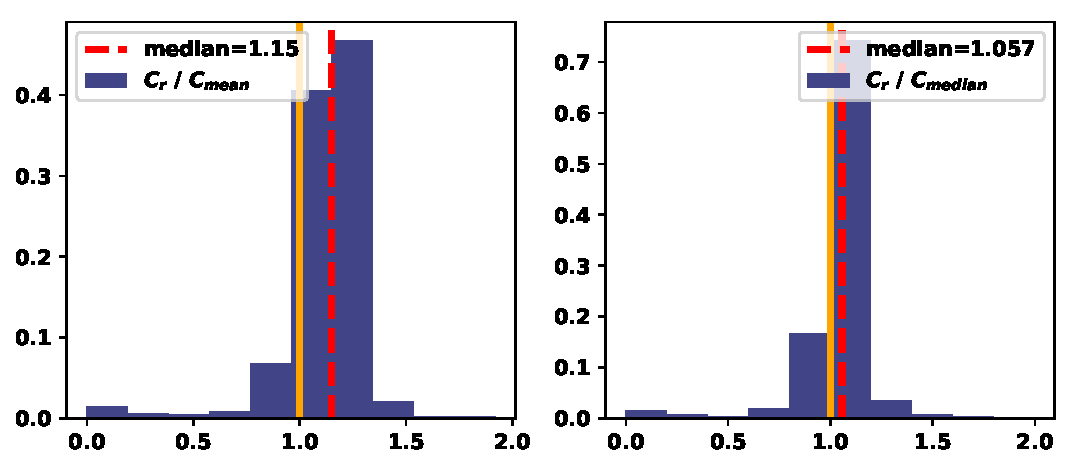
\includegraphics[width=.7\textwidth]{../images/compared_to_mean_median_standard.pdf}
    \caption{Distributions of \(C_r / C_{\text{median}}\)
    and \(C_r / C_{\text{median}}\) for standard tournaments.}\label{fig:mean_median_std}
\end{figure}

\begin{figure}[!htbp]
    \centering
    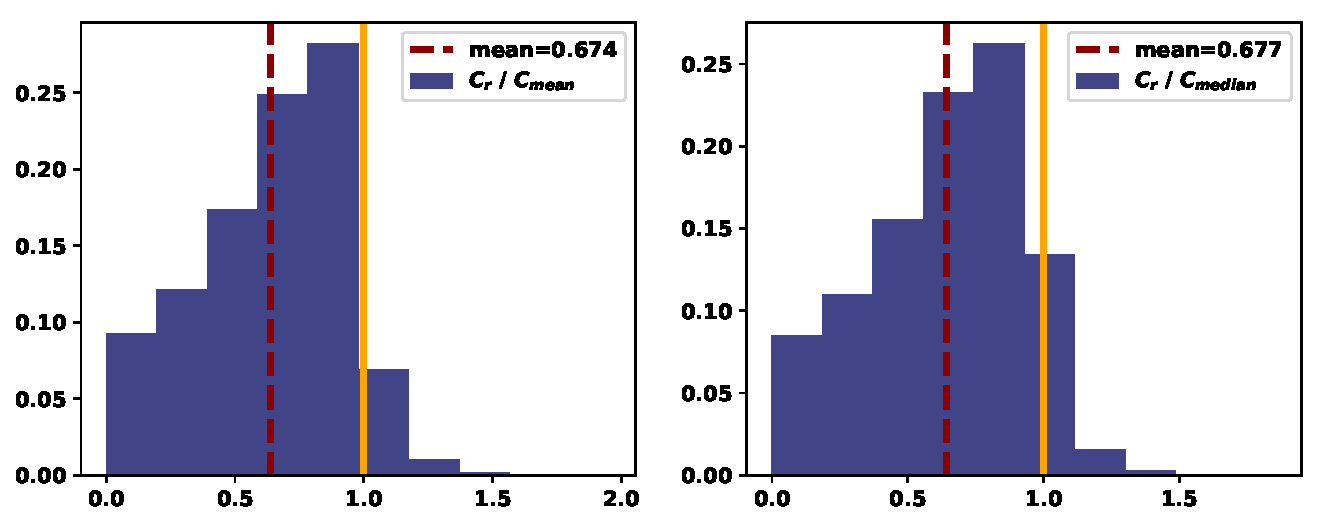
\includegraphics[width=.7\textwidth]{../images/compared_to_mean_median_noisy.pdf}
    \caption{Distributions of \(C_r / C_{\text{median}}\)
    and \(C_r / C_{\text{median}}\) for noisy tournaments.}\label{fig:mean_median_noisy}
\end{figure}

\begin{figure}[!htbp]
    \centering
    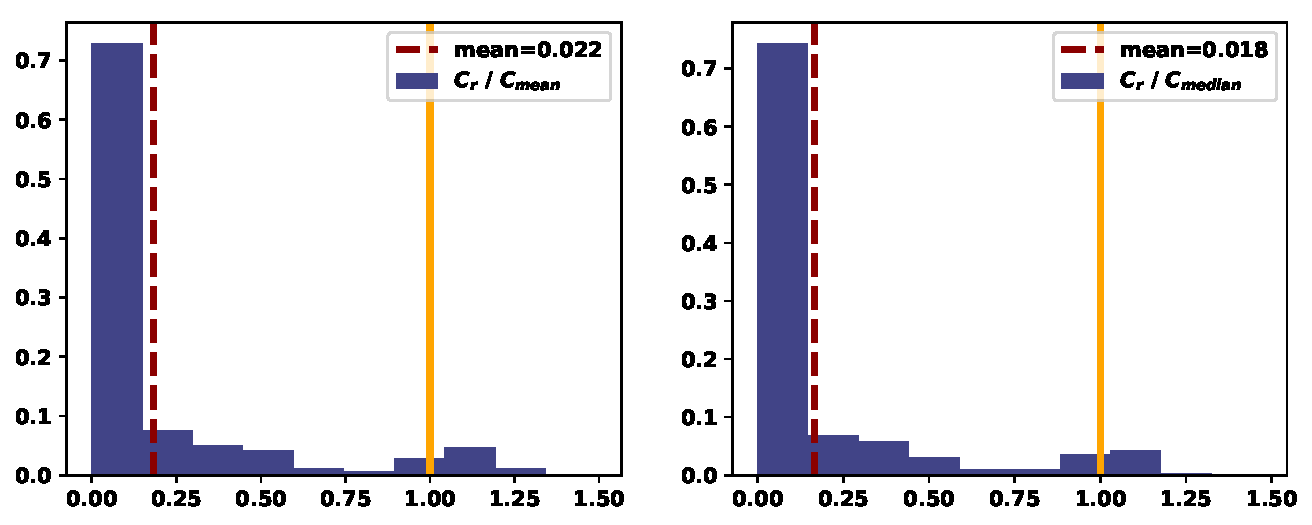
\includegraphics[width=.7\textwidth]{../images/compared_to_mean_median_probend.pdf}
    \caption{Distributions of \(C_r / C_{\text{median}}\)
    and \(C_r / C_{\text{median}}\) for probabilistic ending tournaments.}\label{fig:mean_median_probend}
\end{figure}

\begin{figure}[!htbp]
    \centering
    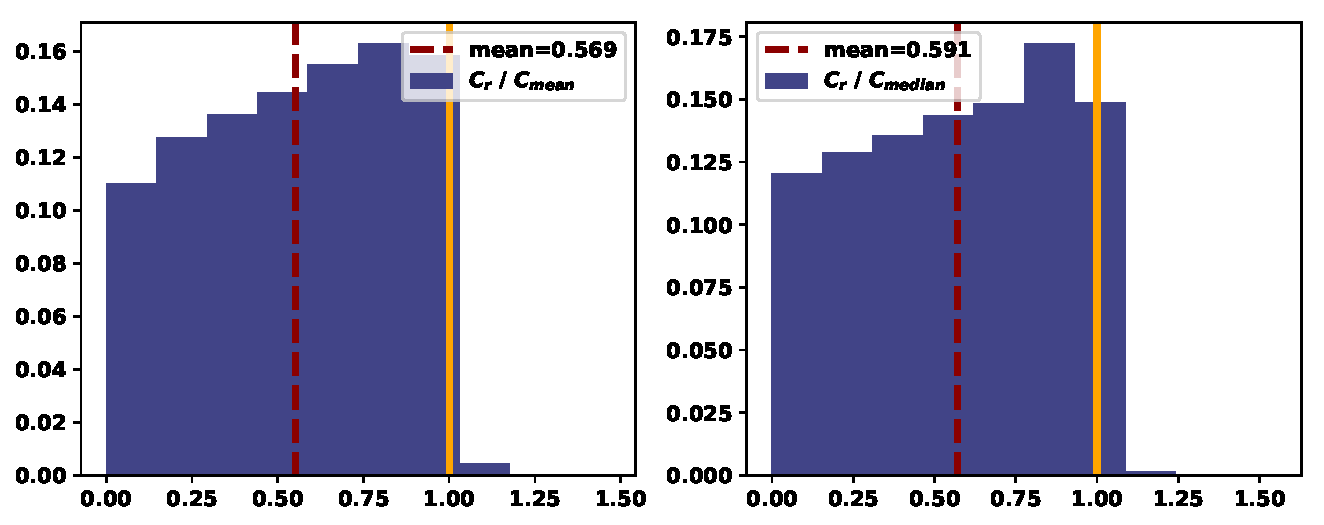
\includegraphics[width=.7\textwidth]{../images/compared_to_mean_median_probend_noisy.pdf}
    \caption{Distributions of \(C_r / C_{\text{median}}\)
    and \(C_r / C_{\text{median}}\) for noisy probabilistic ending tournaments.}\label{fig:mean_median_probend_noisy}
\end{figure}

\begin{figure}[!htbp]
    \centering
    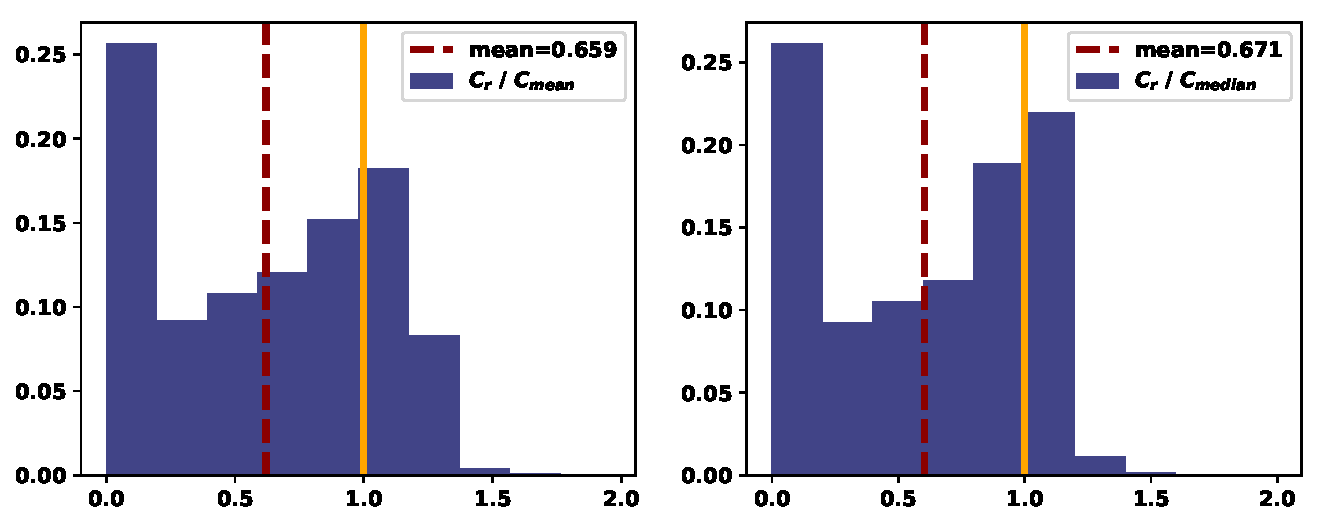
\includegraphics[width=.7\textwidth]{../images/compared_to_mean_median_overall.pdf}
    \caption{Distributions of \(C_r / C_{\text{median}}\)
    and \(C_r / C_{\text{median}}\) for over all the tournaments.}\label{fig:mean_median_overall}
\end{figure}

The factors which have an effect on the performances were presented here by two
approaches which included the correlation coefficients and a random forest
analysis. The results of these are discussed in the following section.

\section{Conclusion}\label{section:conclusion}

This manuscript explored a variety of strategic behaviours in the game of the
Iterated Prisoner's Dilemma and presented an evaluation of performance in the
game. A large number of computer tournaments have been analysis and demonstrated
that a single dominant strategy does not exist in the game. Moreover, it
was shown that from a series of factors that a strategy has control over the
tge factors that can influence it's performance is the cooperating ratio compared
to that of it's environment.

A total of 186 strategies were used in this manuscript, which are available via
an open source software, the Axelrod-Python. By making use of the software a
total of 49,140 computer tournaments results were gathered. In
Section~\ref{section:top_performances}, the result summaries were used to
present the top performances. This was not done over the entire data set. The
data set contains results from four different settings, and these were also
studied individually. The top performances were presented for all the different
combinations of the results summary. Though Retaliate set of families,
strategies introduced in~\cite{axelrodproject}, did perform well in noisy
environments and this feature allowed the strategies to rank well in more than
one tournament type, the analysis concluded that there is not a single dominant
strategy in the Iterated Prisoner's Dilemma. THough a dominant perform
was not highlighted by the analysis of this manuscript the factors that made
performances successful were further explored.

In Section~\ref{section:evaluation_of_performance} an analysis of strategies
features was covered. The results of this analysis showed that a strategy's
characteristics such as it's stochasticity and the information it used regarding
the game had no effect on the strategy's success. The most important
factors have been those that compared the strategy's behaviour to it's environment.
The cooperating ratio of the strategy compared to the mean and median cooperator
was highlighted as the most important feature in the analysis. More specifically,
if a strategy were to enter a tournament with a theory of mind of it's environment
it would choose to be the median cooperator in standard tournaments, the
defector in probabilistic ending tournaments and to cooperate 60\% of the median
in noisy and noisy probabilistic tournaments. Lastly, if a strategy was
aware of the opponents but not of the setting on the tournament, a strategy
would be more likely to be successful if it were to identify the median
cooperator and cooperated 60\% of the times that they did.




\bibliographystyle{plain}
\bibliography{bibliography}

\appendix

\section{List of strategies}\label{app:list_of_players}

The strategies used in this study which are from Axelrod version 3.0.0
\cite{axelrodproject}.

\begin{multicols}{3}
	\begin{enumerate}
		\item $\phi$~\cite{axelrodproject}
\item $\pi$~\cite{axelrodproject}
\item $e$~\cite{axelrodproject}
\item ALLCorALLD \cite{axelrodproject}
\item Adaptive~\cite{Li2011}
\item Adaptive Pavlov 2006~\cite{kendall2007iterated}
\item Adaptive Pavlov 2011~\cite{Li2011}
\item Adaptive Tit For Tat: 0.5~\cite{Tzafestas2000}
\item Aggravater~\cite{axelrodproject}
\item Alexei~\cite{lesswrong}
\item Alternator~\cite{Axelrod1981, Mittal2009}
\item Alternator Hunter~\cite{axelrodproject}
\item Anti Tit For Tat~\cite{Hilbe2013}
\item AntiCycler~\cite{axelrodproject}
\item Appeaser~\cite{axelrodproject}
\item Arrogant QLearner~\cite{axelrodproject}
\item Average Copier~\cite{axelrodproject}
\item Backstabber~\cite{axelrodproject}
\item Better and Better~\cite{prison}
\item Bully~\cite{Nachbar1992}
\item Calculator~\cite{prison}
\item Cautious QLearner~\cite{axelrodproject}
\item Champion~\cite{Axelrod1980b}
\item CollectiveStrategy~\cite{Li2009}
\item Contrite Tit For Tat~\cite{Axelrod1995}
\item Cooperator~\cite{Axelrod1981, Mittal2009, Press2012}
\item Cooperator Hunter~\cite{axelrodproject}
\item Cycle Hunter~\cite{axelrodproject}
\item Cycler CCCCCD~\cite{axelrodproject}
\item Cycler CCCD~\cite{axelrodproject}
\item Cycler CCCDCD~\cite{axelrodproject}
\item Cycler CCD~\cite{Mittal2009}
\item Cycler DC~\cite{axelrodproject}
\item Cycler DDC~\cite{Mittal2009}
\item DBS~\cite{Au2006}
\item Davis~\cite{Axelrod1980a}
\item Defector~\cite{Axelrod1981, Mittal2009, Press2012}
\item Defector Hunter~\cite{axelrodproject}
\item Double Crosser~\cite{axelrodproject}
\item Desperate \cite{Van2015}
\item DoubleResurrection~\cite{Eckhart2015}
\item Doubler~\cite{prison}
\item Dynamic Two Tits For Tat~\cite{axelrodproject}
\item EasyGo~\cite{Li2011, prison}
\item Eatherley~\cite{Axelrod1980b}
\item Eventual Cycle Hunter~\cite{axelrodproject}
\item Evolved ANN~\cite{axelrodproject}
\item Evolved ANN 5~\cite{axelrodproject}
\item Evolved ANN 5 Noise 05~\cite{axelrodproject}
\item Evolved FSM 16~\cite{axelrodproject}
\item Evolved FSM 16 Noise 05~\cite{axelrodproject}
\item Evolved FSM 4~\cite{axelrodproject}
\item Evolved HMM 5~\cite{axelrodproject}
\item EvolvedLookerUp1 1 1~\cite{axelrodproject}
\item EvolvedLookerUp2 2 2~\cite{axelrodproject}
\item Eugine Nier~\cite{lesswrong}
\item Feld~\cite{Axelrod1980a}
\item Firm But Fair~\cite{Frean1994}
\item Fool Me Forever~\cite{axelrodproject}
\item Fool Me Once~\cite{axelrodproject}
\item Forgetful Fool Me Once~\cite{axelrodproject}
\item Forgetful Grudger~\cite{axelrodproject}
\item Forgiver~\cite{axelrodproject}
\item Forgiving Tit For Tat~\cite{axelrodproject}
\item Fortress3~\cite{Ashlock2006}
\item Fortress4~\cite{Ashlock2006}
\item GTFT \cite{Gaudesi2016, Nowak1993}
\item General Soft Grudger~\cite{axelrodproject}
\item Gradual~\cite{Beaufils1997}
\item Gradual Killer~\cite{prison}
\item Grofman\cite{Axelrod1980a}
\item Grudger~\cite{Axelrod1980a, Banks1990, Beaufils1997, Van2015, Li2011}
\item GrudgerAlternator~\cite{prison}
\item Grumpy~\cite{axelrodproject}
\item Handshake~\cite{Robson1990}
\item Hard Go By Majority~\cite{Mittal2009}
\item Hard Go By Majority: 10~\cite{axelrodproject}
\item Hard Go By Majority: 20~\cite{axelrodproject}
\item Hard Go By Majority: 40~\cite{axelrodproject}
\item Hard Go By Majority: 5~\cite{axelrodproject}
\item Hard Prober~\cite{prison}
\item Hard Tit For 2 Tats~\cite{Stewart2012}
\item Hard Tit For Tat~\cite{PD2017}
\item Hesitant QLearner\cite{axelrodproject}
\item Hopeless~\cite{Van2015}
\item Inverse~\cite{axelrodproject}
\item Inverse Punisher~\cite{axelrodproject}
\item Joss~\cite{Axelrod1980a, Stewart2012}
\item Knowledgeable Worse and Worse~\cite{axelrodproject}
\item Level Punisher~\cite{Eckhart2015}
\item Limited Retaliate 2~\cite{axelrodproject}
\item Limited Retaliate 3~\cite{axelrodproject}
\item Limited Retaliate~\cite{axelrodproject}
\item MEM2~\cite{Li2014}
\item Math Constant Hunter~\cite{axelrodproject}
\item Meta Hunter Aggressive~\cite{axelrodproject}
\item Meta Hunter~\cite{axelrodproject}
\item Meta Majority~\cite{axelrodproject}
\item Meta Majority Finite Memory~\cite{axelrodproject}
\item Meta Majority Long Memory~\cite{axelrodproject}
\item Meta Majority Memory One~\cite{axelrodproject}
\item Meta Minority~\cite{axelrodproject}
\item Meta Mixer~\cite{axelrodproject}
\item Meta Winner~\cite{axelrodproject}
\item Meta Winner Deterministic~\cite{axelrodproject}
\item Meta Winner Ensemble~\cite{axelrodproject}
\item Meta Winner Finite Memory~\cite{axelrodproject}
\item Meta Winner Long Memory~\cite{axelrodproject}
\item Meta Winner Memory One~\cite{axelrodproject}
\item Meta Winner Stochastic~\cite{axelrodproject}
\item NMWE Deterministic~\cite{axelrodproject}
\item NMWE Finite Memory~\cite{axelrodproject}
\item NMWE Long Memory~\cite{axelrodproject}
\item NMWE Memory One~\cite{axelrodproject}
\item NMWE Stochastic~\cite{axelrodproject}
\item Naive Prober~\cite{Li2011}
\item Negation~\cite{PD2017}
\item Nice Average Copier~\cite{axelrodproject}
\item Nice Meta Winner~\cite{axelrodproject}
\item Nice Meta Winner Ensemble~\cite{axelrodproject}
\item Nydegger~\cite{Axelrod1980a}
\item Omega TFT~\cite{kendall2007iterated}
\item Once Bitten~\cite{axelrodproject}
\item Opposite Grudger~\cite{axelrodproject}
\item PSO Gambler 1 1 1~\cite{axelrodproject}
\item PSO Gambler 2 2 2~\cite{axelrodproject}
\item PSO Gambler 2 2 2 Noise 05~\cite{axelrodproject}
\item PSO Gambler Mem1 \cite{axelrodproject}
\item Predator~\cite{Ashlock2006}
\item Prober~\cite{Li2011}
\item Prober 2~\cite{prison}
\item Prober 3~\cite{prison}
\item Prober 4~\cite{prison}
\item Pun1~\cite{Ashlock2006}
\item Punisher~\cite{axelrodproject}
\item Raider~\cite{Ashlock2014}
\item Random Hunter~\cite{axelrodproject}
\item Random: 0.5~\cite{Axelrod1980a, Tzafestas2000}
\item Remorseful Prober~\cite{Li2011}
\item Resurrection~\cite{Eckhart2015}
\item Retaliate 2~\cite{axelrodproject}
\item Retaliate 3~\cite{axelrodproject}
\item Retaliate~\cite{axelrodproject}
\item Revised Downing~\cite{Axelrod1980a}
\item Ripoff~\cite{Ashlock2008}
\item Risky QLearner~\cite{axelrodproject}
\item SelfSteem~\cite{Andre2013}
\item ShortMem ~\cite{Andre2013}
\item Shubik~\cite{Axelrod1980a}
\item Slow Tit For Two Tats~\cite{axelrodproject}
\item Slow Tit For Two Tats 2~\cite{prison}
\item Sneaky Tit For Tat~\cite{axelrodproject}
\item Soft Go By Majority~\cite{Axelrod1981, Mittal2009}
\item Soft Go By Majority 10~\cite{axelrodproject}
\item Soft Go By Majority 20~\cite{axelrodproject}
\item Soft Go By Majority 40~\cite{axelrodproject}
\item Soft Go By Majority 5~\cite{axelrodproject}
\item Soft Grudger~\cite{Li2011}
\item Soft Joss~\cite{prison}
\item SolutionB1~\cite{Ashlock2015}
\item SolutionB5~\cite{Ashlock2015}
\item Spiteful Tit For Tat~\cite{prison}
\item Stalker~\cite{Carvalho2013}
\item Stein and Rapoport~\cite{Axelrod1980a}
\item Stochastic Cooperator~\cite{Adami2013}
\item Stochastic WSLS~\cite{axelrodproject}
\item Suspicious Tit For Tat~\cite{Beaufils1997, Hilbe2013}
\item TF1~\cite{axelrodproject}
\item TF2~\cite{axelrodproject}
\item TF3~\cite{axelrodproject}
\item Tester~\cite{Axelrod1980b}
\item ThueMorse~\cite{axelrodproject}
\item ThueMorseInverse~\cite{axelrodproject}
\item Thumper~\cite{Ashlock2008}
\item Tit For 2 Tats (\textbf{Tf2T})~\cite{Axelrod1981}
\item Tit For Tat (\textbf{TFT})~\cite{Axelrod1980a}
\item Tricky Cooperator~\cite{axelrodproject}
\item Tricky Defector~\cite{axelrodproject}
\item Tullock~\cite{Axelrod1980a}
\item Two Tits For Tat (\textbf{2TFT})~\cite{Axelrod1981}
\item VeryBad~\cite{Andre2013}
\item Willing \cite{Van2015}
\item Win-Shift Lose-Stay (\textbf{WShLSt})~\cite{Li2011}
\item Win-Stay Lose-Shift (\textbf{WSLS})~\cite{Kraines1989, Nowak1993, Stewart2012}
\item Winner12~\cite{mathieu2017}
\item Winner21~\cite{mathieu2017}
\item Worse and Worse\cite{prison}
\item Worse and Worse 2\cite{prison}
\item Worse and Worse 3\cite{prison}
\item ZD-Extort-2 v2~\cite{Kuhn2017}
\item ZD-Extort-2~\cite{Stewart2012}
\item ZD-Extort-4~\cite{axelrodproject}
\item ZD-GEN-2~\cite{Kuhn2017}
\item ZD-GTFT-2~\cite{Stewart2012}
\item ZD-SET-2~\cite{Kuhn2017}
	\end{enumerate}
\end{multicols}

\section{Acknowledgements}

A variety of software have been used in this work:

\begin{itemize}
    \item The Axelrod library for IPD simulations~\cite{axelrodproject}.
    \item The Matplotlib library for visualisation~\cite{hunter2007matplotlib}.
    \item The Numpy library for data manipulation~\cite{walt2011numpy}.
    \item The scikit-learn library for data analysis~\cite{scikit-learn}.
\end{itemize}

\end{document}